\documentclass[12pt, a4paper]{report}
\usepackage{style}
\usepackage{makecell}

\title{Software Engineering II \\ \textit{Theory}}
\author{Christian Rossi}
\date{Academic Year 2023-2024}

\begin{document}

\maketitle

\newpage

\begin{abstract}
    The objective of the course is to teach the principals methods and processes of software engineering needed to develop complex and qualitative software.
     
    The course covers the following arguments:
    \begin{itemize}
        \item Software process and its organization.
        \item Modelling languages.
        \item Requirements analysis and definition.
        \item Software development methods and tools.
        \item Approaches for verify and validate the software.
    \end{itemize}
\end{abstract}

\newpage

\tableofcontents

\newpage

\chapter{Introduction}
    \section{Definition}
    The realm of software engineering is dedicated to unraveling the multitude of challenges that emerge during the creation of extensive software systems.
    These systems are inherently intricate due to their substantial scale, the collaboration of individuals from diverse fields, and the necessity for continuous adjustments to meet evolving demands (both during development and post-installation). 
    \begin{definition}
        \emph{Software engineering} is a methodical and managerial discipline that revolves around the systematic creation and upkeep of software products, all of which are crafted and sustained within predefined, controlled timeframes and cost constraints.
    \end{definition}
    In contrast to traditional programming, where a programmer typically crafts an entire piece of software based on known specifications independently, software engineers embark on a distinct path.
    They identify requirements, shape specifications, design components meant to interconnect with others, and engage in collaborative efforts within a team setting. 
    The key competencies of a software engineer encompass technical acumen, managerial prowess, cognitive aptitude, and organizational skills.

    \section{History}
    In its early days, software was regarded as an art form. 
    Computers primarily served the purpose of mathematical problem-solving, with the designers themselves acting as the end users. 
    The initial programs were crafted using low-level languages and were subject to stringent resource constraints.
    
    However, as the demand for customized software surged, this artistic endeavor transitioned into a more methodical craft. 
    Developers began creating programs tailored for a broader audience, employing new high-level languages.
    Towards the culmination of this era, a "software crisis" loomed, marked by the escalating complexity of software and a dearth of effective software development techniques.

    With the intention of tackling this growing challenge, the term was coined during a NATO conference in 1968. 
    The primary focus of this pivotal gathering encompassed the following key areas:
    \begin{itemize}
        \item Development of software and the establishment of standards.
        \item Strategic planning and proficient management.
        \item Automation of software development processes.
        \item Modularization of software design.
        \item Rigorous quality assurance and verification.
    \end{itemize}

    \section{The process and product}
    The creation of a software program necessitates a well-defined process. 
    Both the software itself and the procedures employed possess inherent quality, and it is imperative for the software engineer to strive for the highest quality possible. 
    This is essential because the process directly influences the ultimate outcome.
    
    Software distinguishes itself from conventional product types in several ways, as it is:
    \begin{enumerate}
        \item Intangible, making it challenging to precisely describe and evaluate.
        \item Adaptable or malleable, capable of being modified to suit evolving requirements.
        \item Human-intensive, devoid of straightforward manufacturing processes.
    \end{enumerate}
    Software quality is influenced by various critical factors, including development technology, process quality, the caliber of individuals involved, cost considerations, and adherence to predefined schedules. 
    Software quality attributes encompass:
    \begin{itemize}
        \item Correctness: ensuring that the software aligns with specified requirements.
        \item Reliability: minimizing the probability of failure absence over a defined period.
        \item Robustness: assessing the software's ability to perform reasonably in unforeseen scenarios.
        \item Performance: evaluating the efficient utilization of resources.
        \item Usability: focusing on the ease of use for the anticipated user base.
        \item Maintainability: the capacity to facilitate software maintenance.
        \item Reusability: extending maintainability to components, promoting their reuse.
        \item Portability: the adaptability of software to diverse target environments.
        \item Interoperability: ensuring harmonious coexistence and cooperation with other applications.
    \end{itemize}
    Process quality attributes consist of:
    \begin{itemize}
        \item Productivity: assessing the efficiency and output of the development process.
        \item Unity of effort (person-month): measuring the collective contribution of effort over a month.
        \item Delivered item (lines of code and function points): quantifying the tangible output of the development process.
        \item Timeliness: the capability to respond to change requests in a timely fashion.
    \end{itemize}

    \section{Development process}
    In the initial stages of software development, there was a lack of reference models, leading to a straightforward "code and fix" approach. 
    In response to the previously mentioned software crisis, the necessity for a structured model became evident.
    The first comprehensive model introduced was the "waterfall" model, characterized by the following fundamental requirements:
    \begin{enumerate}
        \item Identification of distinct phases and associated activities.
        \item Enforcement of a linear progression, with no backtracking between phases.
        \item Standardization of outputs generated at each phase.
        \item Viewing software development as akin to a manufacturing process.
    \end{enumerate}
    Following the advent of the waterfall model, numerous more flexible methodologies emerged, including iterative models, the agile movement, and DevOps, which aimed to offer more adaptable approaches to software development.
    \begin{figure}[H]
        \centering
        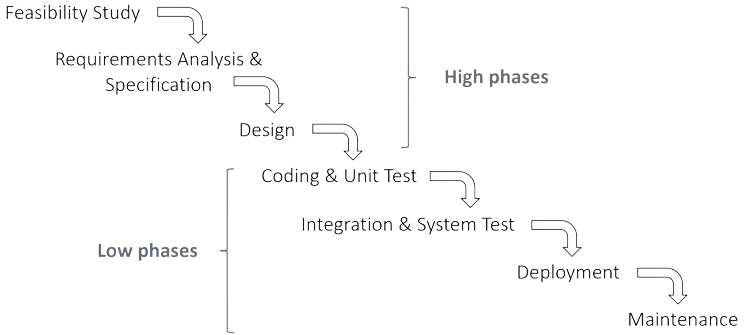
\includegraphics[width=0.75\linewidth]{images/waterfall.png}
        \caption{Waterfall process model}
    \end{figure}
    The key phases depicted in the image encompass the following:
    \begin{enumerate}
        \item Feasibility study and project estimation: this stage determines whether the project should commence, exploring possible alternatives and necessary resources. 
            It yields a "feasibility study document" comprising an initial problem description, scenarios outlining potential solutions, and cost and schedule estimates for various options.
        \item Requirement analysis and specification: in this phase, the domain in which the application operates is meticulously analyzed. 
            Requirements are identified, and software specifications are derived, leading to the creation of a "requirement analysis and specification document". 
        \item Design: this step outlines the software architecture, defining components, their relationships, and interactions. 
            The objective is to facilitate concurrent development and allocate responsibilities. 
            It culminates in the production of a "design document". 
        \item Coding and unit test: each module is implemented and rigorously tested. 
            Additional quality assurance measures, such as inspections, may be employed. 
            Programs are accompanied by their respective documentation.
        \item Integration and system test: modules are integrated into systems, and the integrated systems undergo testing. 
            This phase, as well as the preceding one, can be integrated into an incremental implementation scheme.
        \item Deployment.
        \item Maintenance; the maintenance phase comprises various aspects, including:
            \begin{itemize}
                \item Corrective: addressing and rectifying identified faults or defects.
                \item Adaptive: adapting the software to changes in its environment.
                \item Perfective: accommodating new or modified user requirements.
                \item Preventive: involving activities aimed at enhancing the system's maintainability.
            \end{itemize}
    \end{enumerate}
    \begin{figure}[H]
        \centering
        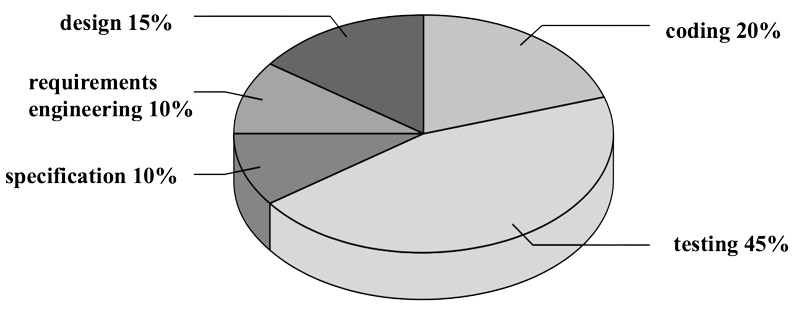
\includegraphics[width=0.75\linewidth]{images/effort.png}
        \caption{Effort in each phase}
    \end{figure}
    
    The primary challenges associated with software evolution include:
    \begin{itemize}
        \item It is seldom anticipated and strategically planned.
        \item Software is highly amenable to change, with modifications often directly affecting the code, leading to inconsistencies in project documentation.
    \end{itemize}
    Effectively addressing software evolution necessitates the implementation of sound engineering practices, comprising two key steps: first, modifying the design, and then making corresponding adjustments in the implementation, ensuring the consistent updating of all associated documents.
    Indeed, one of the central objectives of software engineering is to create software that can be designed to accommodate future changes in a dependable and cost-effective manner.

    The waterfall model operates as a black-box system, as the company seeking the software provides initial requirements and remains relatively uninvolved throughout the development phase. 
    If a higher degree of transparency and customer interaction is required, an alternative development model must be adopted, one that permits regular customer feedback. With each customer interaction, two key aspects can be evaluated:
    \begin{itemize}
        \item Validation: ensuring that the product aligns with the customer's specific requests.
        \item Verification: confirming that the product functions correctly and in the intended manner.
    \end{itemize}
    The concept of a flexible development process is centered on its adaptability to changes, particularly in requirements and specifications.
    This approach involves incremental processes that allow for feedback at various stages.
    There are various forms of flexible development processes, such as SCRUM, extreme programming, incremental releases, rapid prototyping, DevOps, and more.

\newpage

\chapter{Requirements engineering}
    \section{Definition}
    The primary measure of success of a software system is the degree to which it meets the purpose for which it was intended.
    \begin{definition}
        Software systems \emph{requirements engineering} is the process of discovering that purpose, by identifying stakeholders and their needs, and documenting these in a form that is amenable to analysis, communication, and subsequent implementation. 
    \end{definition}
    This phase entails pivotal considerations: stakeholder identification, needs assessment, documentation generation, and the analysis, communication, and implementation of requirements. 
    An alternate definition is as follows:
    \begin{definition}
        \emph{Requirements engineering} is the branch of software engineering concerned with the real-world goals for, function of, and constraints on software systems. 
        It is also concerned with the relationship of these factors to precise specifications of software engineering behavior, and to their evolution over time and across software families. 
    \end{definition}

    \section{Importance and difficulties}
    Customer-provided requirements can be categorized into three primary types:
    \begin{itemize}
        \item Functional requirements: These delineate the system's interactions with its environment, irrespective of implementation details. 
            They represent the core objectives that the software must achieve.
        \item Nonfunctional requirements: These encompass user-visible aspects of the system that aren't directly tied to functional behavior.
        \item Constraints: these restrictions are either set by the client or are inherent to the system's operational environment.
    \end{itemize}
    Nonfunctional requirements, often referred to as quality of service attributes, specify how functionality should be delivered to the end user. 
    While they transcend specific application domains, their relevance and prioritization are influenced by the application's context.
    \begin{figure}[H]
        \centering
        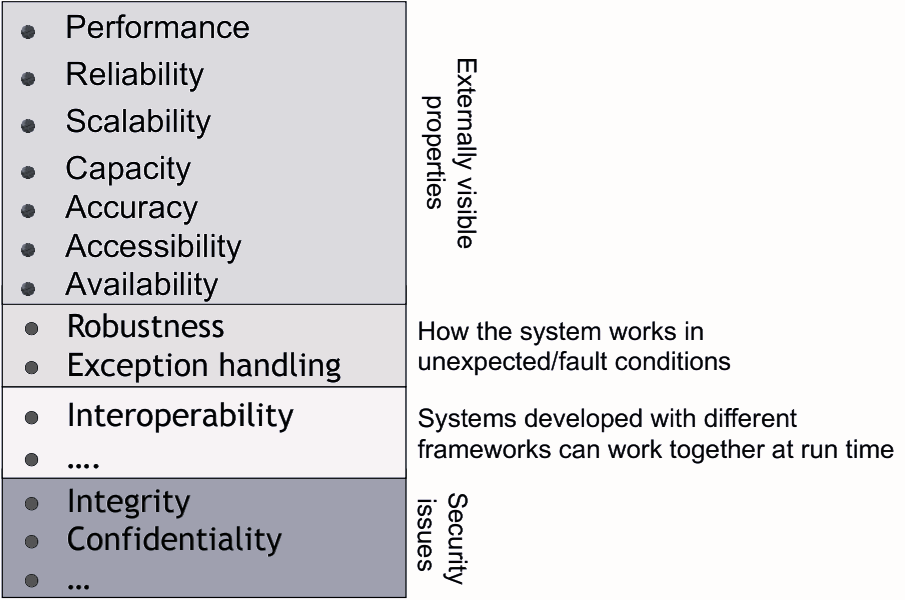
\includegraphics[width=0.5\linewidth]{images/QoS.png}
        \caption{Some relevant QoS characteristics}
    \end{figure}

    \section{Requirement engineering process}
    Inadequate requirements are widespread, and the process of requirement engineering is both challenging and pivotal. 
    This is because issues in the initial stages can potentially escalate costs by a factor of up to two hundred during the final phase.
    \begin{figure}[H]
        \centering
        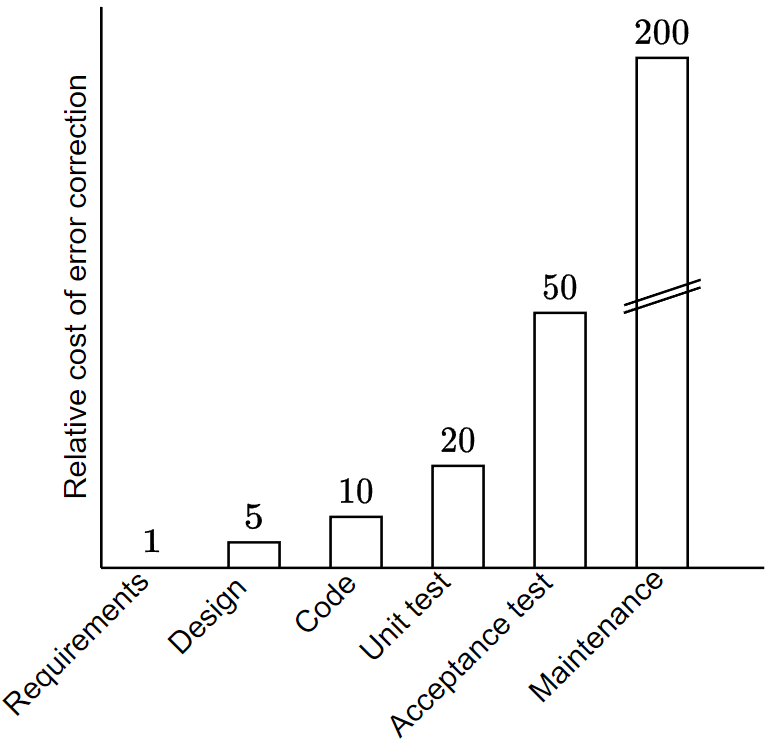
\includegraphics[width=0.5\linewidth]{images/requirements.png}
        \caption{Cost of late correction [Boehm, 1981]}
    \end{figure}
    The complexity of requirement engineering arises from several factors, including composite systems, the presence of multiple systems, varying abstraction levels, diverse concerns, and involvement of stakeholders with different backgrounds.
    
    Requirement engineers are tasked with various responsibilities, including:
    \begin{itemize}
        \item Eliciting information, which involves gathering details about project objectives, context, scope, domain boundaries, and requirements.
        \item Modeling and analysis, encompassing the definition of goals, objects, use cases, and scenarios.
        \item Communicating requirements, which includes providing analysis feedback, documenting in the Requirements Analysis and Specification Document (RASD), and creating system prototypes.
        \item Negotiating and agreeing upon requirements, which involves resolving conflicts and managing risks, assisting in requirement selection and prioritization.
        \item Managing and evolving requirements, involves overseeing them across the entire development lifecycle, ensuring backward and forward traceability, and effectively managing changes and their consequences.
    \end{itemize}

    \section{World-machine relationship}
    The machine signifies the portion of the system to be developed, while the world denotes the segment of the real-world influenced by the machine. 
    It is crucial to note that the machine's purpose always resides within the context of the world.
    
    Requirements engineering is primarily concerned with phenomena occurring in the world, rather than those confined to the machine itself. 
    In essence, requirements models serve as representations of real-world phenomena.
     
    Certain phenomena are shared between the world and the machine. 
    These shared phenomena fall into two categories:
    \begin{itemize}
        \item Phenomena controlled by the world and observed by the machine.
        \item Phenomena controlled by the machine and observed by the world.
    \end{itemize}
    \begin{figure}[H]
        \centering
        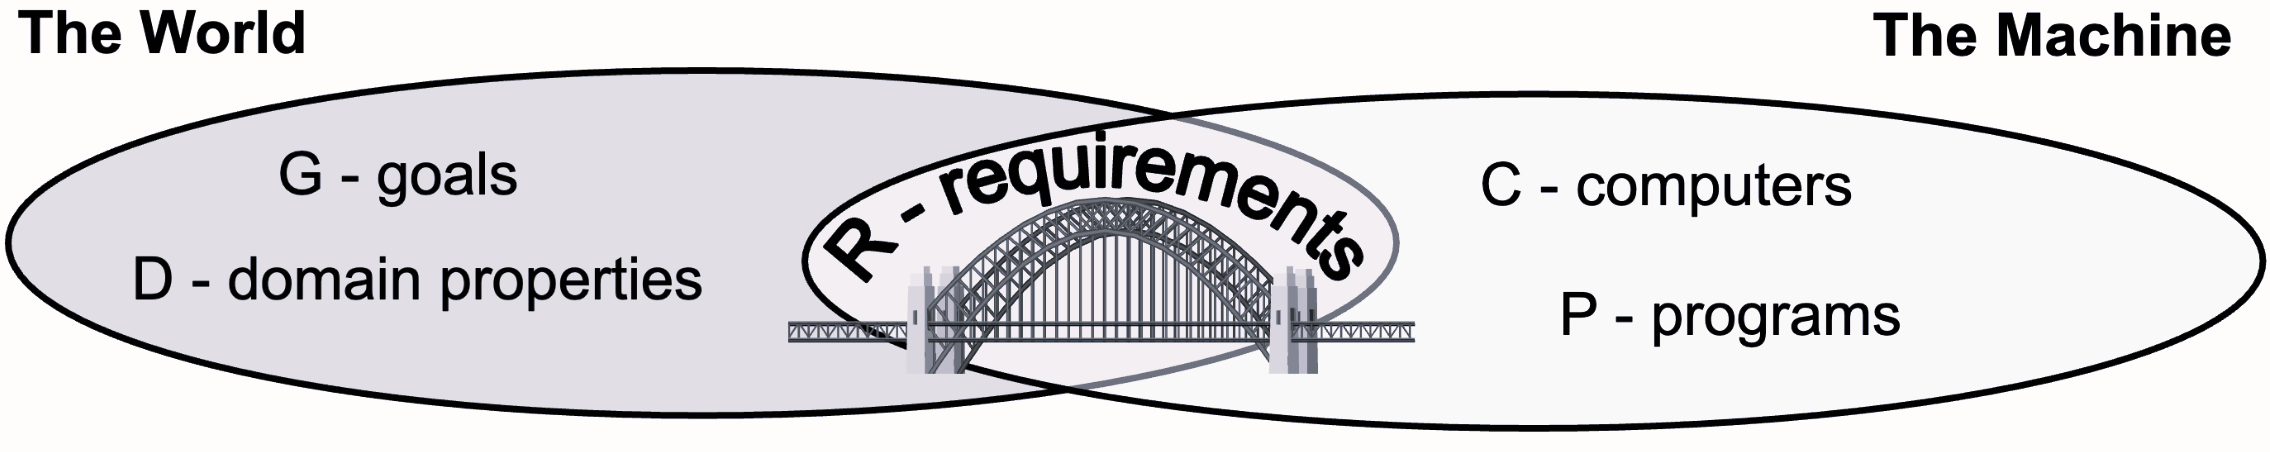
\includegraphics[width=0.75\linewidth]{images/worldmachine.png}
        \caption{Goals, domain assumptions, and requirements}
    \end{figure}
    Goals are declarative statements formulated in terms of real-world phenomena, which may or may not be shared.
    Domain properties and assumptions, on the other hand, are descriptive statements presumed to be valid in the world. 
    Requirements, as prescriptive assertions, are expressed in terms of shared phenomena.
      
    The completeness of requirements, denoted as $R$, is achieved if:
    \begin{itemize}
        \item $R$ guarantees the satisfaction of goals $G$ within the context of domain properties $D$, expressed as $R\land D \models G$.
        \item $G$ comprehensively capture all the needs of stakeholders.
        \item $D$ accurately represent valid properties and assumptions about the world.
    \end{itemize}

    \section{Elicitation of requirements}
    The complexity in requirement engineering can be managed through various means, including:
    \begin{itemize}
        \item Employing diverse approaches and strategies, and synthesizing the outcomes from each.
        \item Maintaining proximity to stakeholders.
        \item Enabling stakeholders to articulate their perspectives.
    \end{itemize}
    This scenario can be generalized in terms of:
    \begin{itemize}
        \item Involving participation actors.
        \item Defining entry conditions.
        \item Outlining the flow of events.
        \item Specifying exit conditions.
        \item Identifying exceptional cases.
        \item Documenting special requirements.
    \end{itemize}

    \section{Modeling requirements}
    \begin{definition}
        A \emph{model} is a depiction, typically in one medium, of an entity in the same or a different medium.
        It encapsulates the essential facets of the subject while simplifying or omitting extraneous details.
    \end{definition}
    Reality, denoted as $R$, comprises tangible entities, individuals, processes, and their interconnections. 
    In contrast, a model, symbolized as $M$, represents an abstraction of these entities, individuals, processes, and the relationships between these abstractions.
    
    To comprehend reality, it necessitates interpretation denoted as $I$ through a mapping function.
    For a model to be considered effective, it is imperative that the relationships that hold true in reality $R$ also hold true in the model $M$.
    \begin{figure}[H]
        \centering
        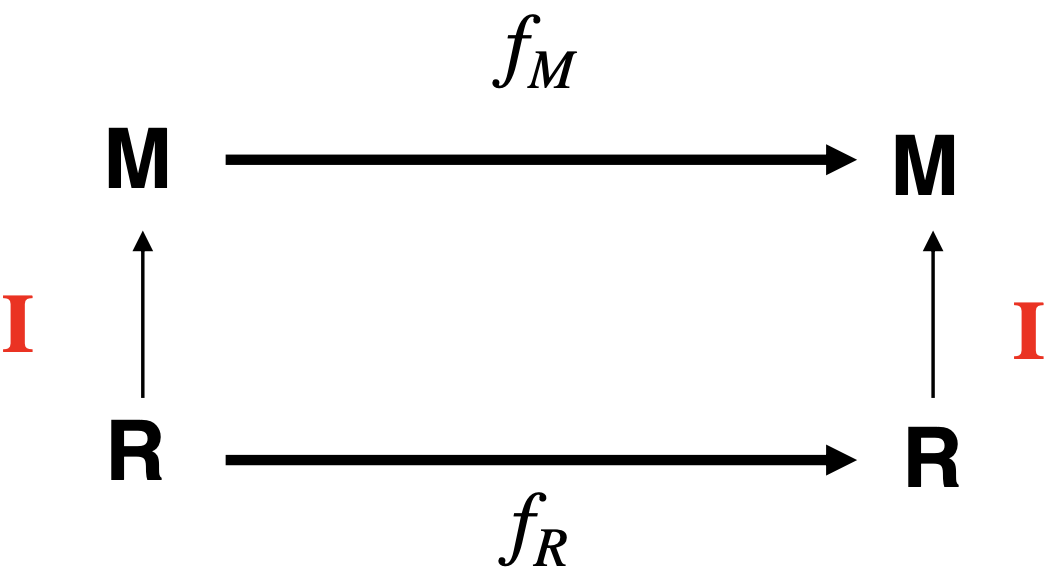
\includegraphics[width=0.5\linewidth]{images/modeling.png}
        \caption{Relationship between model $M$ and reality $R$}
    \end{figure}
    Software models serve a variety of purposes, including:
    \begin{itemize}
        \item Capturing and articulating requirements and domain knowledge with precision.
        \item Facilitating software system design and the generation of practical deliverables.
        \item Offering a simplified perspective on intricate systems and enabling evaluation and simulation of such complexity.
        \item Generating prospective system configurations.
    \end{itemize}
    The primary modeling challenges revolve around ensuring coherence among different perspectives of the system and addressing the potential for variations in interpretation and ambiguity by establishing clear boundaries for acceptable differences in how the model is understood.
     
    In the domain of requirements engineering, our modeling efforts should primarily focus on:
    \begin{itemize}
        \item Representing the pertinent entities and individuals relevant to the given problem.
        \item Describing the relevant phenomena.
        \item Documenting the objectives, requirements, and domain assumptions.
    \end{itemize}
    When it comes to choosing the appropriate modeling tools, we have several options at our disposal:
    \begin{itemize}
        \item Natural language (e.g., English, Italian, etc.):
            \begin{itemize}
                \item Pros: user-friendly and easy to use.
                \item Cons: prone to a high level of ambiguity, and it's possible to overlook relevant information.
            \end{itemize}
        \item Formal language (e.g., FOL, Alloy, Z, etc.):
            \begin{itemize}
                \item Pros: offers the possibility of employing tools for analysis and validation; this approach compels the user to specify all crucial details.
                \item Cons: requires expertise in using the language.
            \end{itemize}
        \item Semiformal language (e.g., UML):
            \begin{itemize}
                \item Pros: simpler than a formal language, providing some degree of structure to the models.
                \item Cons: not amenable for automated analysis, and still entails some level of ambiguity.
            \end{itemize}
        \item Mixed approach:             
            \begin{itemize}
                \item Utilizing a semiformal language for foundational aspects.
                \item Augmenting semiformal models with explanatory informal text.
                \item Leveraging a formal language for the most critical components.
            \end{itemize}
    \end{itemize}
    The choice of the modeling tool should align with the specific requirements and characteristics of the project at hand.

    \section{Use cases and requirements}
    The fundamental steps in formulating use cases encompass the following:
    \begin{enumerate}
        \item Assign a name to the use case.
        \item Identify the actors: generalize specific names to encompass participating actors.
        \item Focus on the flows of events, entry and exit conditions using natural language.
        \item Give due attention to exceptional cases and special requirements.
    \end{enumerate}
    Each use case can give rise to one or more requirements.
     
    A use case represents a sequence of events within the system, involving interactions with actors. 
    These use cases are initiated by an actor and conclude under specific termination conditions.
    \begin{definition}
        The \emph{use case model} is the set of all use cases specifying the complete functionality of the system. 

        A \emph{use case association} is a relationship between use cases. 
        The primary types of use case associations include:
        \begin{itemize}
            \item Include, where one use case utilizes another use case.
            \item Extends, where a use case extends the behavior of another use case.
            \item Generalization, when an abstract use case has several specialized versions.
        \end{itemize}
    \end{definition}
    \begin{figure}[H]
        \centering
        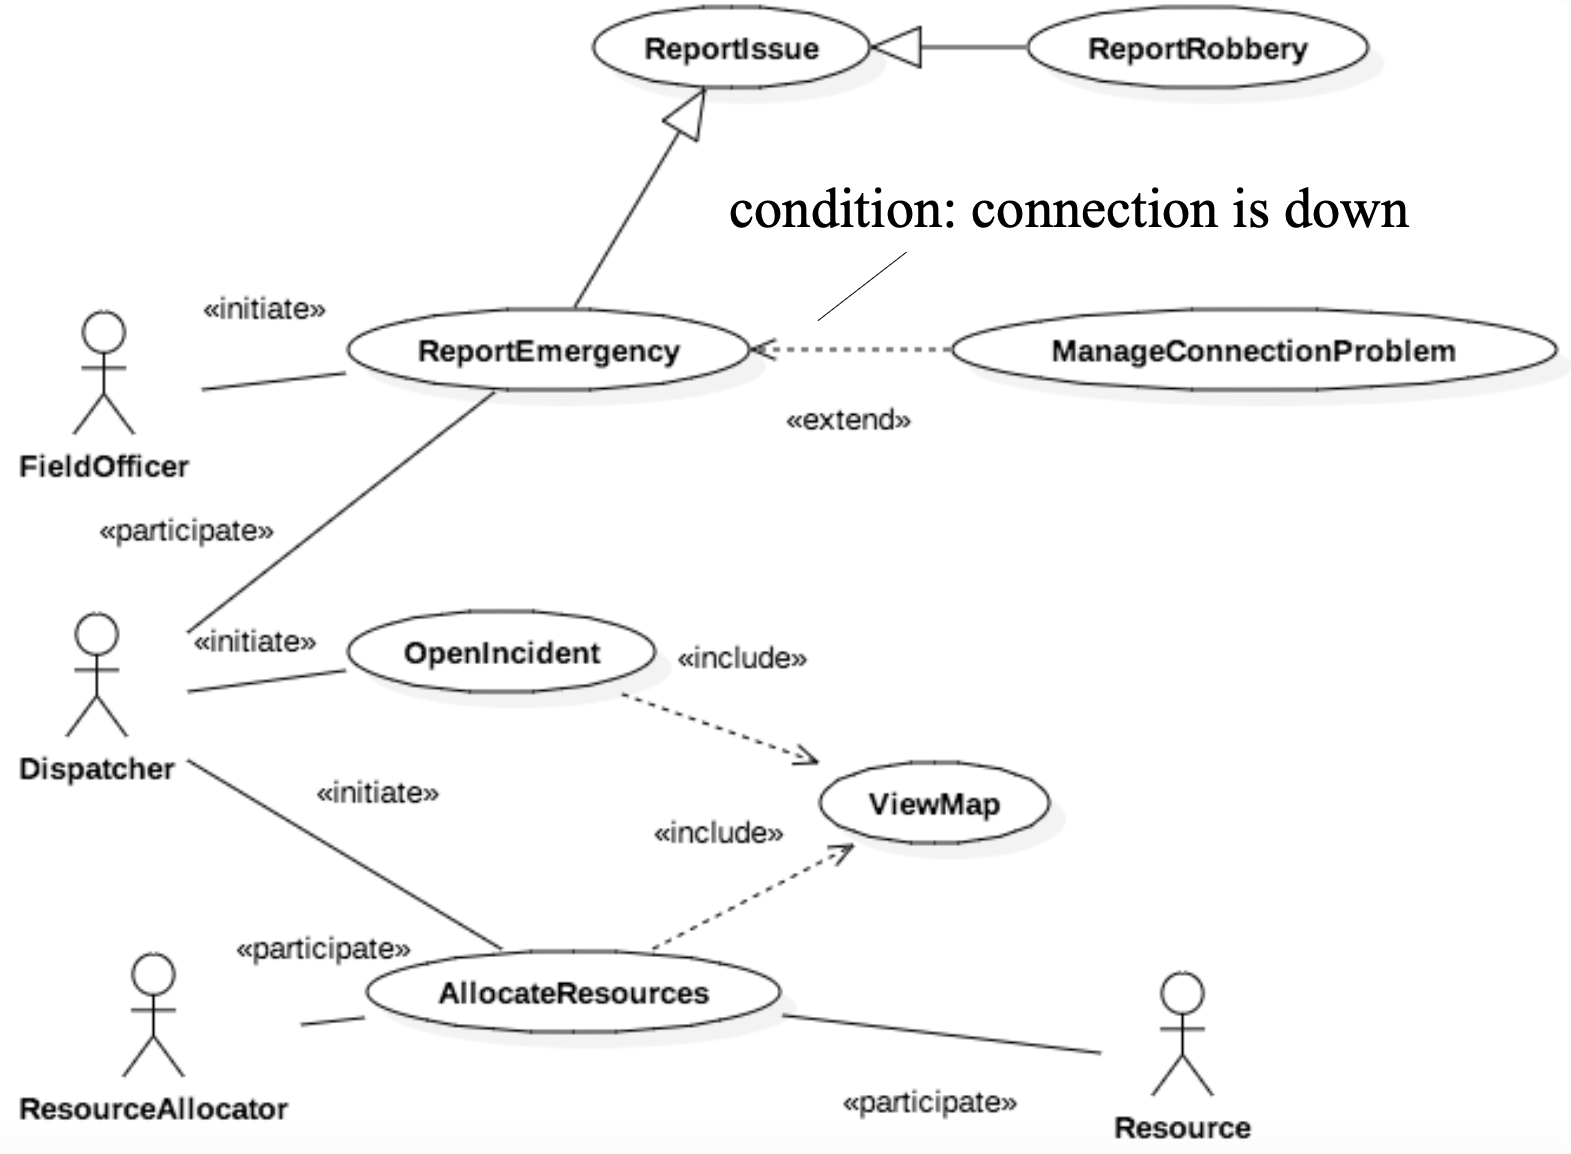
\includegraphics[width=0.6\linewidth]{images/usecase.png}
        \caption{Use case model example}
    \end{figure}

    \section{Requirements-level class diagrams}
    The requirements-level class diagrams are conceptual models for the application domain. They may model objects that will not be represented in the software-to-be. Usually, they 
    do not attach operations to objects: it's best to postpone this kind of decisions until software design. 
     
    To find objects and classes we need to:
    \begin{itemize}
        \item Analyze any description of the problem and application domain you may have.
        \item Analyze your scenarios and use cases descriptions.
    \end{itemize}
    Finding objects is the central piece in object modeling. A possible tool to use in the analysis is the Abbott Textual Analysis also called noun-verb analysis: nouns are good 
    candidates for classes and verbs are good candidates for associations and operations. 
    \begin{table}[H]
        \centering
        \begin{tabular}{ccc}
        \textbf{Example}                  & \textbf{Grammatical construct} & \textbf{UML component} \\ \hline
        "Monopoly"                        & concrete person, thing         & object                 \\
        "toy"                             & noun                           & class                  \\ \hline
        "3 years old"                     & adjective                      & attribute              \\ \hline
        "enters"                          & verb                           & operation              \\
        "depends on"                      & intransitive verb              & operation (event)      \\ \hline
        "is a", "either", "or", "kind of" & classifying verb               & inheritance            \\ \hline
        "has a", "consists of"            & possessive verb                & aggregation            \\ \hline
        "must be", "less than"            & modal verb                     & constraint             \\ \hline
        \end{tabular}
        \caption{Abbott textual analysis example}
    \end{table}

    \section{Dynamic modeling}
    Dynamic modeling serves the purpose of providing methodologies for modeling interactions, the behavior of participants, and workflow within a system. 
    This is achieved through various diagram types, including sequence diagrams, state machine diagrams, and activity diagrams. 
    During the creation of these diagrams, certain objects become apparent.
     
    A sequence diagram is established by following the flow of events outlined in the use case diagram. 
    It represents objects engaged in a use case scenario using a directed acyclic graph notation. 
    The fundamental rules for creating sequence diagrams include:
    \begin{itemize}
        \item Every event involves both a sender and a receiver.
        \item The representation of the event is sometimes referred to as a message.
        \item The sender and receiver for each event must be identified.
    \end{itemize}
    \begin{figure}[H]
        \centering
        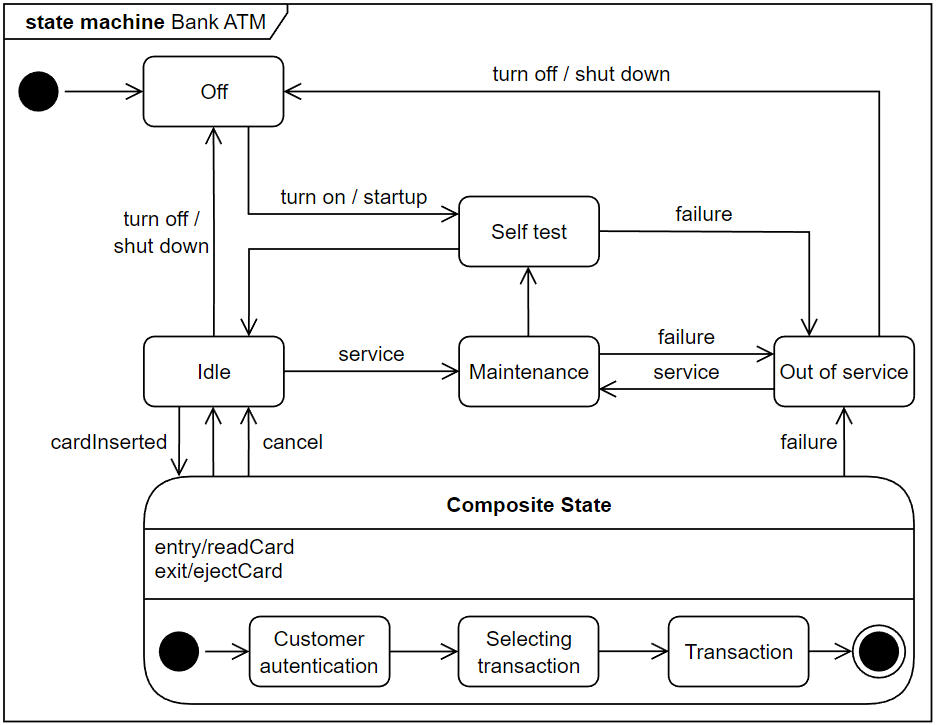
\includegraphics[width=0.5\linewidth]{images/state.png}
        \caption{Example of a state diagram}
    \end{figure}
    For effective dynamic modeling, it is crucial to construct models solely for classes exhibiting substantial dynamic behavior, considering only relevant attributes. 
    Additionally, when deciding on actions and activities, one must account for the granularity of the application and strive to reduce notational complexity.

\newpage

\chapter{Alloy}
    \section{Introduction}
    Alloy is a formal notation designed for specifying models of both systems and software. 
    It exhibits characteristics akin to a declarative object-oriented language, underpinned by a robust mathematical foundation.   
    To aid in the practical application of Alloy, a supporting tool is available, facilitating the simulation of specifications and enabling property verification.
    
    Alloy has been crafted with the objective of combining the expressive power found in the Z language with the rigorous automated analysis capabilities offered by the SMW model checker.
    In the realm of requirement engineering, Alloy finds utility in formally describing the domain, its inherent properties, or the operations that a machine is required to provide.
    In software design, Alloy serves as a valuable tool for the formal modeling of components and their interdependencies.    

    Alloy represents a fusion of first-order logic and relational calculus. 
    Key features of this formal language include:
    \begin{itemize}
        \item A thoughtfully curated subset of relational algebra, offering a uniform model for individuals, sets, and relations, with an absence of high-order relations.
        \item Minimal reliance on arithmetic operations.
        \item Support for modules and hierarchies to enhance organization and scalability.
        \item Designed for succinct, illustrative specifications.
        \item Employs a potent and efficient analysis tool.
    \end{itemize}
    
    \section{Syntax}
    Alloy presents bounded snapshots of the world that satisfy the given specification. 
    
    It employs bounded exhaustive search to uncover counterexamples to asserted properties using SAT.        
    \newpage
    \begin{definition}
            \emph{Atoms} represent Alloy's fundamental entities, characterized by indivisibility, immutability, and a lack of interpretation.

            \emph{Relations} establish connections between atoms, forming sets of tuples, where tuples are sequences of atoms.
        \end{definition}
        In Alloy, relations are inherently typed, with their types determined by the declaration of the relation. 
        The fundamental Alloy relation types include:
        \begin{itemize}
            \item "none" (signifying an empty set). 
            \item "univ" (representing the universal set).
            \item "iden" (denoting the identity relation).
        \end{itemize}
        The logical operators in Alloy encompass:
        \begin{itemize}
            \item Union "$\cup$".
            \item Intersection "$\&$".
            \item Difference "$-$".
            \item Subset "$in$".
            \item Equality "$=$".
            \item Cross product "$\rightarrow$", analogous to a natural join.
            \item Dot join "$.$" or "$[\:]$", where the final element of the first relation joins with the corresponding first elements of the second relation, followed by the removal of the combined element from the relation.
        \end{itemize}
        Here are the various binary closures applicable to relations in Alloy:
        \begin{itemize}
            \item Transpose "$\sim$": inverts the order of the elements in the relation.
            \item Transitive "$\land$": it signifies the transitive closure where $^{\land}r=r+r.r+r.r.r+\dots$. 
            \item Reflexive transitive "$*$": it represents the reflexive transitive closure, where $^{*}r=\textnormal{iden}+^{\land}r$. 
        \end{itemize}
        The possible restrictions are: 
        \begin{itemize}
            \item Domain restriction "$<:$", that restricts the elements on the left side to the set on the right side.
            \item Range restriction "$:>$", that is same as before, but the relations are inverted. 
            \item Override "$++$", that removes the tuples on the left that are in the right relations and adds all the remaining relations of the right relation. 
        \end{itemize}
        Alloy also includes various Boolean operators:
        \begin{itemize}
            \item Negation ("$!$" or "not"). 
            \item Conjunction ("$\&$" or "and"). 
            \item Disjunction ("$\mid \mid$" or "or"). 
            \item Implication ("$\implies$" or "implies"). 
            \item Alternative ("$,$" or "else"). 
            \item Bi-Implication ("$\iff$" or "iff").
        \end{itemize}
        Alloy offers logic quantifiers:
        \begin{itemize}
            \item "all": holds for every element.
            \item "some": holds for at least one element.
            \item "no": holds for no elements.
            \item "lone": holds for at most one element.
            \item "one": holds for exactly one element.
        \end{itemize}
        For defining relations with singletons, you can use the following declaration "x: m e", where "x" is the name of the relation, "m" is the multiplicity of the element (e.g., "set", "one", "lone", or "some") and "e" is the name of the element within the relation. 
        When the relation consists of pairs, the declaration appears as "r: Am $\rightarrow$ nB", where "r" is the relation name, "A" and "B" denote the element names with multiplicities "m" and "n", respectively.
         
        Additionally, Alloy includes operators like "$\#$" (counting the number of tuples in $r$), integers ($0,1,\dots$) for defining variable values, arithmetic operators ("$+$" and "$-$"), and various comparison operators ("$<$", "$<=$", "$=$", "$=>$", "$>$"). 
        There is also the "sum" operator, which adds all elements within a selected tuple.
        
        Other useful keywords are: 
        \begin{itemize}
            \item "let:" this keyword is utilized to establish local variables within a formula or expression. 
                These variables serve to store and reuse intermediate results, making it easier to simplify complex expressions.
            \item "enum": this keyword is employed to define enumerations. 
                Enumerations enable the definition of a finite set of symbolic values, which can be utilized in models to represent various states, options, or categories.
            \item "var": this keyword is used for declaring variables within an Alloy model or specification.
            \item "after": this keyword is employed to specify the temporal ordering or sequence of events or states within a model. 
                It is commonly used in temporal logic to define the sequence of events that must occur before or after a specific state or action.
            \item "always": this keyword is used to express a property that must remain true throughout a system's execution or under certain conditions.
                It is often utilized to specify invariant properties in Alloy models.
            \item "eventually": this keyword is used to express temporal logic properties that indicate a particular condition or event will ultimately occur during the execution of a system. 
                It is commonly used to model and verify properties that describe what should happen at some point in the future.
            \item "historically": keyword is used to express temporal logic properties that describe a condition or event that has remained true for a continuous duration of time leading up to the present or to a specified point in the model's execution.
                It is often employed to specify properties related to the historical behavior of a system.
            \item "before". 
            \item "once".
        \end{itemize}

        \section{Address book example}
        Let's consider the task of creating a basic address book model. 
        This address book contains a collection of addresses associated with their respective names.
        In this scenario, there are three primary entities:
        \begin{itemize}
            \item "Name": represents names of individuals.
            \item "Addr": represents addresses.
            \item "Book": signifies the context of the address book.
        \end{itemize}
        The relationship here is established through the entity "Addr", which links "Name" to "Addr" within the context of "Book". 
        We use the "lone" keyword to indicate that each "Name" can be linked to at most one "Addr". To summarize the preceding descriptions:
        \begin{lstlisting}[language=alloy]
sig Name {}
sig Addr {}
sig Book {
    addr: Name -> lone Addr
}
        \end{lstlisting}
        This specification creates the following relationships: 
        \begin{itemize}
            \item Sets are unary relations.
            \item Scalars are sets consisting of a single element.
            \item The ternary relation involves these three predicates.
        \end{itemize}
        A new predicate can be defined using the "pred" keyword.
        \begin{lstlisting}[language=alloy]
pred show {}
run show for 3 but exactly 1 Book
        \end{lstlisting}
        In the second line, it specifies that we should find a maximum of three elements for each "Book". 
        The previously defined predicate "show" is currently empty and always returns true.
        We can now create a predicate with specific arguments. 
        For instance:
        \begin{lstlisting}[language=alloy]
pred show [b:Book]{
    # b.addr > 1
}
run show for 3 but exactly 1 Book
        \end{lstlisting}
        In the previous example, the consistent predicate imposes a restriction on the quantity of "Address" relations within a given "Book". 
        In the following example, the consistent predicate enforces a constraint on the number of distinct "Address" entries that appear within the "Book"
        \begin{lstlisting}[language=alloy]
pred show [b:Book]{
    # b.addr > 1
    # Name.(b.addr) > 1
}
run show for 3 but exactly 1 Book
        \end{lstlisting}
        In the subsequent example, the inconsistent predicate utilizes the "some" keyword, indicating the existence of an element. 
        In this scenario, there is only one "Book" so the tool will report that no instances can be identified.
        \begin{lstlisting}[language=alloy]
pred add [b:Book]{
    # b.addr > 1
    some n:Name | # n.(b.addr) > 1
}
run show for 3 but exactly 1 Book
        \end{lstlisting}
        All the preceding predicates are considered static as they do not modify the signature. 
        In Alloy, dynamic predicates are used for dynamic analysis. 
        For instance, we can create a predicate that introduces an "Address" and a "Name" to a "Book" as follows:
        \begin{lstlisting}[language=alloy]
pred add [b,b':Book, n:Name,a:Addr]{
    b'.addr=b.addr + n -> a
}
pred showAdd [b,b':Book, n:Name,a:Addr]{
    add[b,b',n,a]
    #Name.(b'.addr) > 1
}
run showAdd
        \end{lstlisting}
        We can now define a predicate for the "Book" deletions.  
        \begin{lstlisting}[language=alloy]
pred del [b,b':Book, n:Name]{
    b'.addr=b.addr - n -> Addr
}
        \end{lstlisting}
        We can verify whether performing a delete operation after an add operation restores us to the initial state or not by employing an "assertion". 
        \begin{lstlisting}[language=alloy]
assert delRevertsAdd{
    all b1,b2,b3:Book,n:Name,a:Addr
    add[b1,b2,n,a] and del[b2,b3,n]
    implies b1.addr=b3.addr
}
        \end{lstlisting}
        During the assertion verification process, Alloy looks for counterexamples. 
        In this instance, we will encounter a counterexample, causing the assertion to evaluate as false.
        To rectify the assertion, we should amend it as follows:
        \begin{lstlisting}[language=alloy]
assert delUndoesAdd{
    all b1,b2,b3:Book,n:Name,a:Addr |
    no n.(b1.addr) and add[b1,b2,n,a] and del[b1,b2,n]
    implies b1.addr=b3.addr
}
        \end{lstlisting}
        In some cases, we may need to retrieve specific signatures. 
        To accomplish this, we can leverage Alloy functions. 
        For instance, we can define a function that searches for a particular "Book" and returns a set of "Address":        
        \begin{lstlisting}[language=alloy]
fun lookup[b:Book,n:Name]: set Addr{
    n.(n.addr)
}
        \end{lstlisting}
    
        \section{Family relations example}
        Now, let's explore a family relationship tree. 
        To begin, we must define a generic individual, which can be either male or female.        
        \begin{lstlisting}[language=alloy]
abstract sig Person {
    father: lone Man
    mother: lone Woman
}
sig Man extends Person {
    wife: lone Woman
}
sig Woman extends Person {
    husband: lone Man
}
        \end{lstlisting}
        We establish that each "Person" can have at most one father and one mother (indicated by the keyword "lone"), as we require a root for the family tree. 
        The person at the root should have no parents, possibly due to them being unknown. 
        The "Person" signature is declared as "abstract" because it needs to be specialized into one of the subsequent signatures, either "Man" or "Woman". 
        Signatures, denoted by the "sig" keyword, represent sets of elements. 
        Before this keyword, we can specify the number of entities required ("lone", "one", or "some").
        \begin{definition}
            The \emph{fields} of a signature are relations whose domain is a subset of the signature. 
            
            The keyword \emph{extends} is used to declare a subset of signature. 
        \end{definition}
        To obtain the set of grandfathers of a given individual, we can define a function like this:
        \begin{lstlisting}[language=alloy]
fun grandpas[p:Person]:set Person {
    p.(mother+father).father
}
pred ownGrandpa[p:Person] {
    p in p.grandpas[p]
}
        \end{lstlisting}
        We've additionally created a predicate that verifies if a person is within the set of grandfathers returned by the "grandpas" function. 
        However, the issue at hand is that we haven't imposed constraints on relations. 
        To address this, we need to define two new operators for binary relations:
        \begin{itemize}
            \item Transitive closure: \textasciicircum $r=r+r.r+r.r.r+\dots$
            \item Reflex transitive closure: $*r=iden+$\textasciicircum$r$
        \end{itemize}
        We can now specify that no one can be their own father or mother:
        \begin{lstlisting}[language=alloy]
fact {
    no p:Person | p in p.^(mother+father)
}
        \end{lstlisting}
        We must also establish a constraint that if X is the husband of Y, then Y is the wife of X:
        \begin{lstlisting}[language=alloy]
fact {
    all m:Man,w:Woman | m.wife=w iff w.husband=m
}
fact {
    wife = ~husband
}
\end{lstlisting}
        The two statements are equivalent, with the second being expressed using the transpose operator.
        A fact can encompass multiple constraints, meaning that the previous constraints can be consolidated into a single fact.
        It's worth noting that facts are global, while predicates need to be invoked explicitly.

\newpage

\chapter{Requirement analysis and specification}
    \section{Structure of a RASD document}
        The Requirements and Specifications Document (RASD) serves several purposes:
        \begin{itemize}
            \item Communication: it conveys an understanding of the requirements, encompassing the application domain and the system under development.
            \item Contractual: it can be legally binding, serving as a formal agreement between stakeholders.
            \item Baseline for project planning and estimation: it provides a foundation for project planning and estimation, covering aspects like size, cost, and schedule.
            \item Baseline for software evaluation: it supports system testing, verification, and validation activities. 
                It contains the information necessary to verify if the delivered system aligns with the requirements.
            \item Baseline for change control: it establishes a foundation for managing changes in requirements as the software evolves.
        \end{itemize}
        The RASD document is utilized by various stakeholders, including:
        \begin{itemize}
            \item Customers and Users: they are interested in a high-level description of system functionalities and requirements.
            \item System analyst and requirement analysts: these individuals use the RASD to specify how the system interacts with other systems.
            \item Developers and programmers: they refer to the RASD for implementation details.
            \item Testers: they use the RASD to check if the system meets its requirements.
            \item Project managers: they rely on the RASD to control the development process.
        \end{itemize}
        \begin{figure}[H]
            \centering
            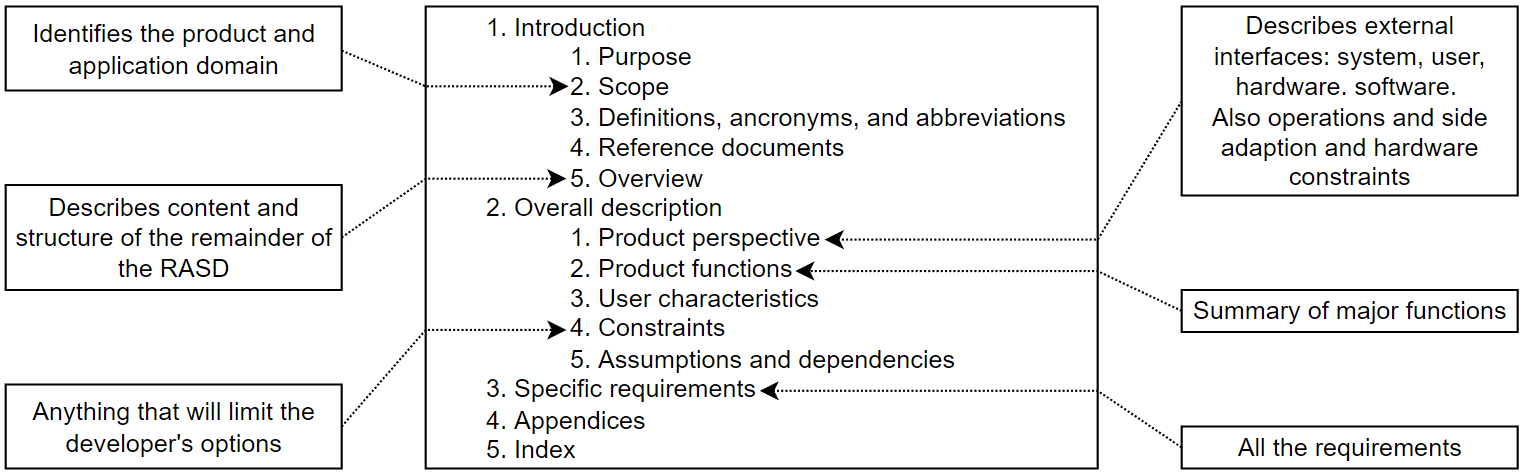
\includegraphics[width=0.75\linewidth]{images/RASD.png}
            \caption{IEEE standard for RASD}
        \end{figure}
         
        A well-crafted RASD should possess the following qualities:
        \begin{itemize}
            \item Completeness:
                \begin{itemize}
                    \item Regarding goals: all requirements must satisfy the goals within specified domain assumptions.
                    \item Regarding inputs: software behavior should be specified for all possible inputs.
                    \item Structural completeness. 
                \end{itemize}
            \item Pertinence: 
                \begin{itemize}
                    \item Each requirement or domain assumption should be necessary for achieving a goal.
                    \item Each goal should be genuinely needed by the stakeholders.
                    \item The RASD should not contain items unrelated to requirement definitions.
                \end{itemize}
            \item Consistency: there should be no contradictions in the formulation of goals, requirements, and assumptions.
            \item Unambiguity: 
                \begin{itemize}
                    \item Clear and well-defined vocabulary.
                    \item Unambiguous assertions. 
                    \item Verifiability of requirements.
                    \item Clear delineation of responsibilities between the software and its environment.
                \end{itemize}
            \item Feasibility: the goals and requirements must be achievable within the allocated budget and schedules.
            \item Comprehensibility: the RASD should be easily understandable by the target audience.
            \item Good structuring: every item must be defined before it is used.
            \item Modifiability: the document should be adaptable, and the impact of modifications should be assessable.
            \item Traceability: 
                \begin{itemize}
                    \item Indication of the sources of goals, requirements, and assumptions.
                    \item Linking requirements and assumptions to underlying goals.
                    \item Facilitating referencing of requirements in future documentation.
                \end{itemize}
        \end{itemize}   
        This structured RASD document ensures effective communication and clarity while serving as a contractual and foundational reference throughout the software development process.


\newpage 

\chapter{Software design}
    \section{Software architecture}
        \begin{definition}
            The \emph{architecture} of a software system defines the system in terms of computational components and the interactions among these components.

            In the context of a software system, the \emph{software architecture} represents the set of structures necessary to reason about the system. 
            These structures include software elements, their relationships, and properties associated with both.
        \end{definition}
        There are three fundamental structures relevant to software architecture:
        \begin{itemize}
            \item Component-and-connector structures: these structures describe how the system is organized as a set of elements with runtime behavior (components) and their interactions (connectors). 
                They allow us to study runtime properties, such as availability and performance, as well as how these structures collaborate.
                \begin{figure}[H]
                    \centering
                    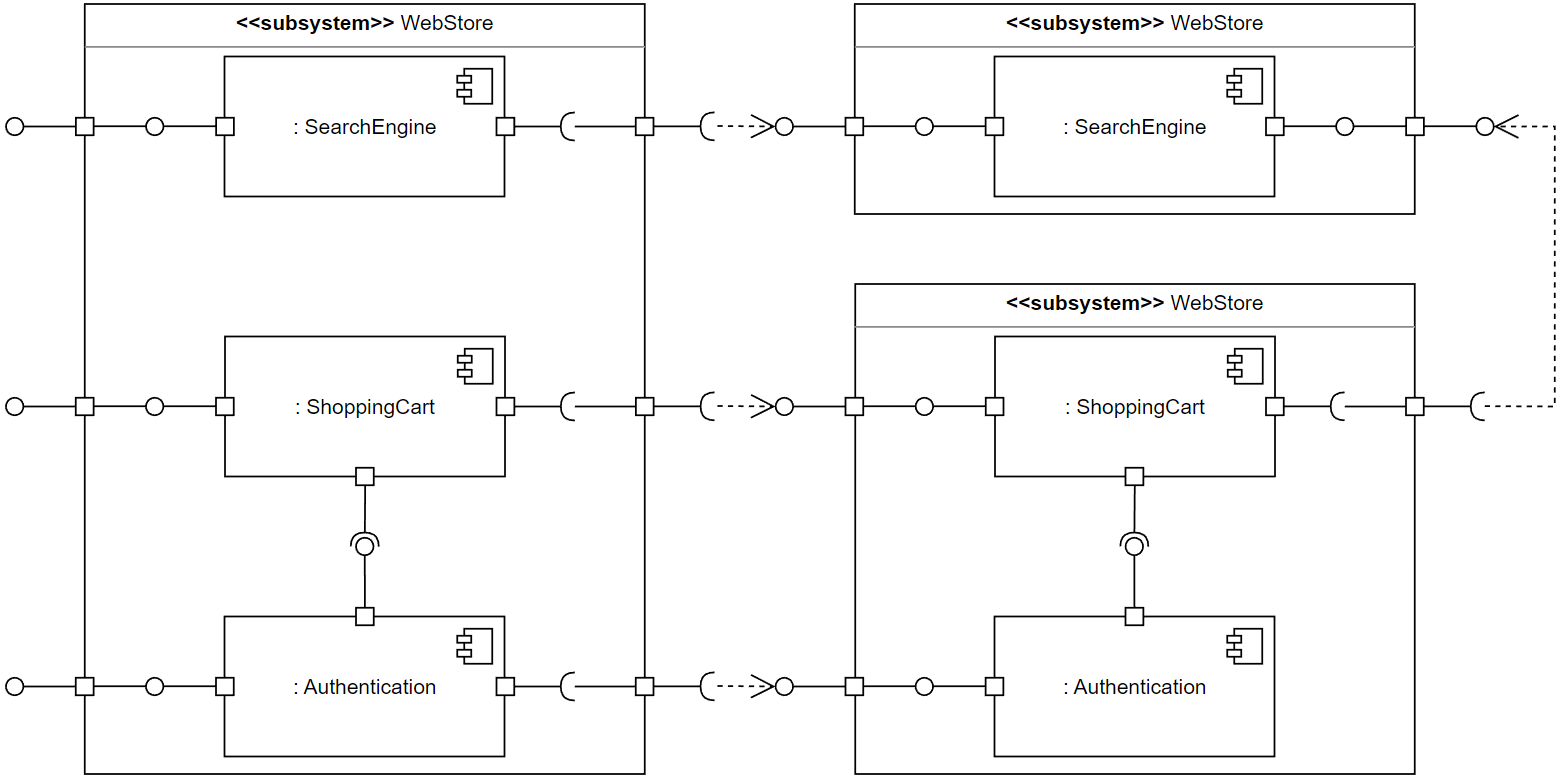
\includegraphics[width=0.75\linewidth]{images/component1.png}
                    \caption{UML component diagrams for component and connector structure}
                \end{figure}
                \begin{figure}[H]
                    \centering
                    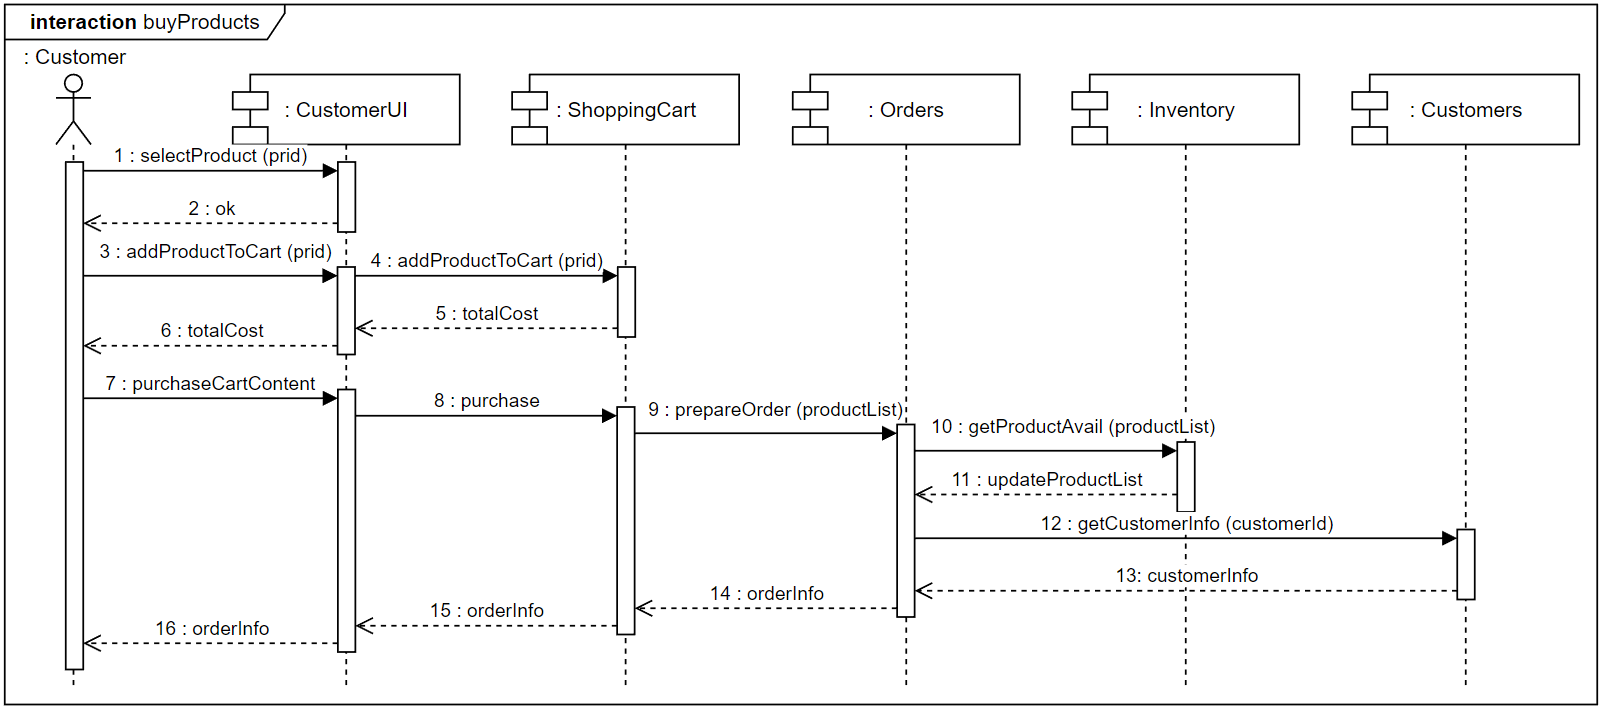
\includegraphics[width=0.75\linewidth]{images/component2.png}
                    \caption{UML sequence diagrams for component and connector structure}
                \end{figure}
            \item Module structures: illustrate how a system is structured as a set of code or data units that need to be procured or constructed, along with their relationships. 
                Modules serve as implementation units and form the basis for work division.
                Typical relationships among these modules include "uses," "is-a" (generalization), and "is-part-of."
                \begin{figure}[H]
                    \centering
                    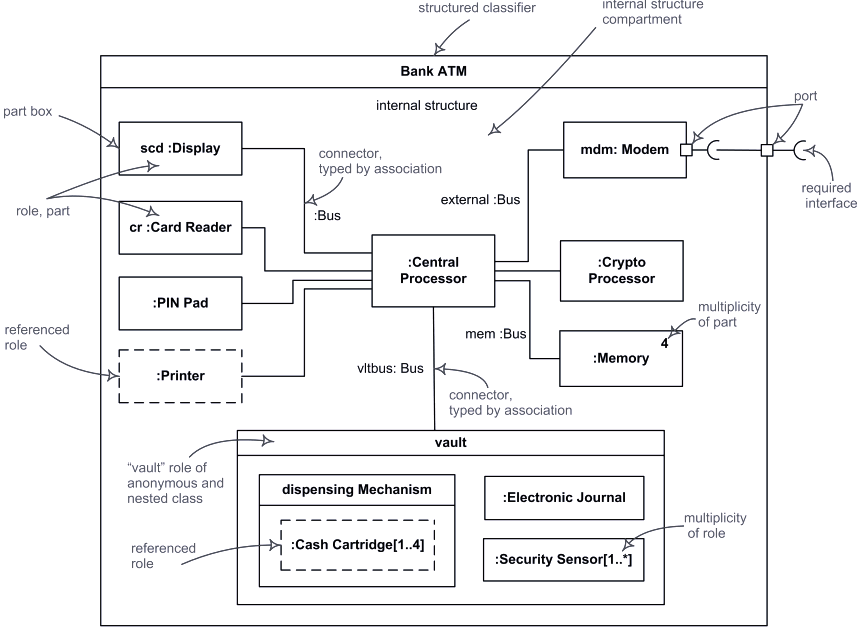
\includegraphics[width=0.4\linewidth]{images/modular1.png}
                    \caption{UML composite structure diagram for module structure}
                \end{figure}
                \begin{figure}[H]
                    \centering
                    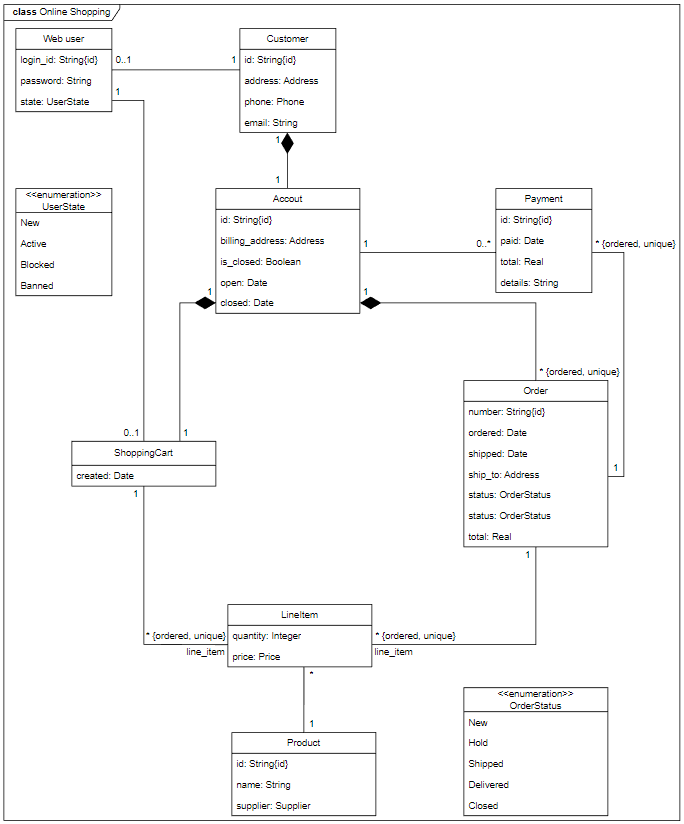
\includegraphics[width=0.4\linewidth]{images/modular2.png}
                    \caption{UML class diagram for module structure}
                \end{figure}
                \begin{figure}[H]
                    \centering
                    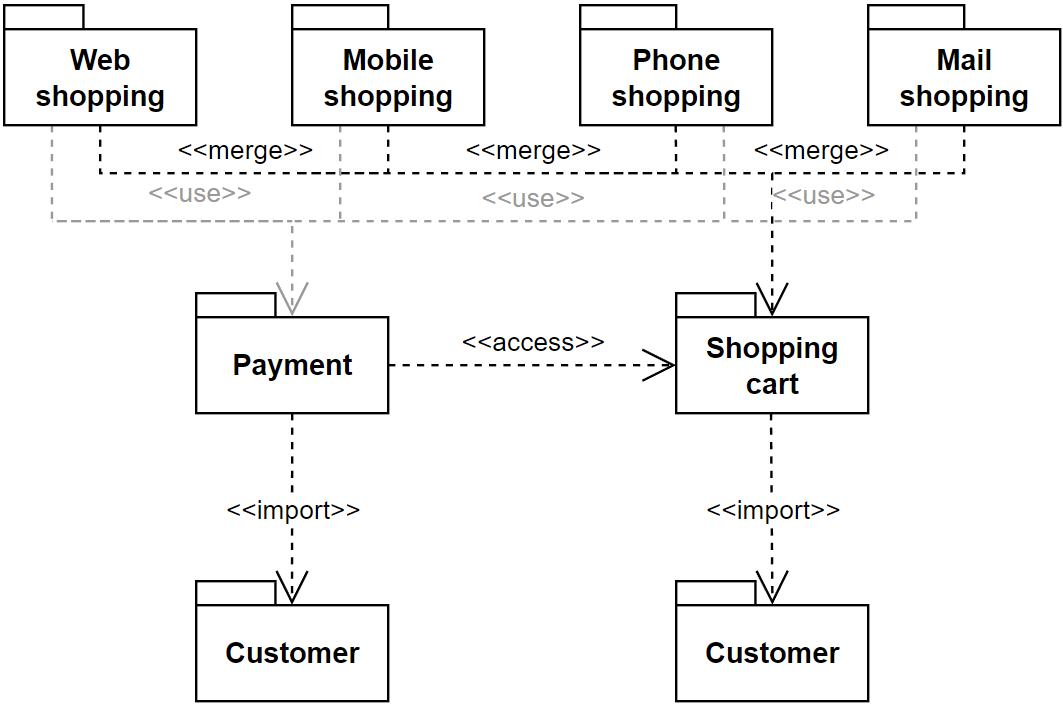
\includegraphics[width=0.4\linewidth]{images/modular3.png}
                    \caption{UML package diagram for module structure}
                \end{figure}
            \item Allocation structures: these structures define how the elements from component and connector or module structures map to entities that are not software. 
                Common allocation structures include deployment structure, implementation structure, and work assignment structure. 
                The deployment structure captures the system's hardware topology, specifying the distribution of components and identifying performance bottlenecks.
                \begin{figure}[H]
                    \centering
                    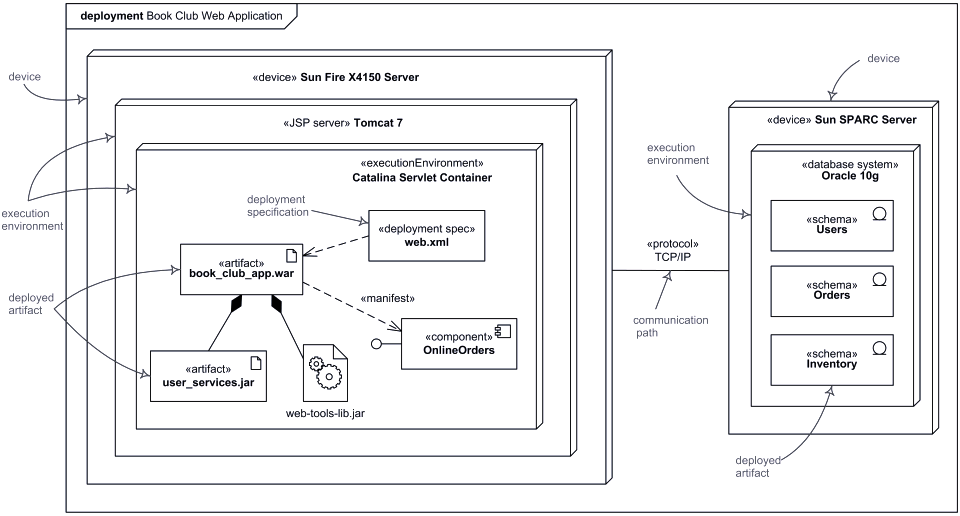
\includegraphics[width=0.5\linewidth]{images/allocation1.png}
                    \caption{UML deployment diagrams and deployment structure}
                \end{figure}
                \begin{figure}[H]
                    \centering
                    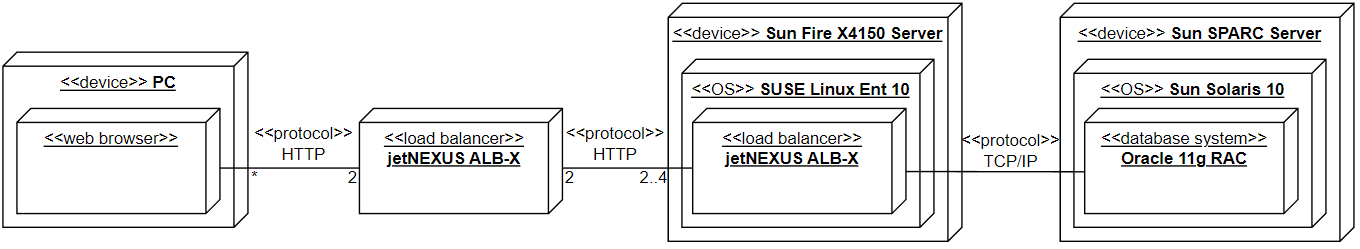
\includegraphics[width=0.5\linewidth]{images/allocation2.png}
                    \caption{UML deployment diagrams and deployment structure}
                \end{figure}
        \end{itemize}

        \subsection{Summary}
        \begin{table}[H]
            \centering
            \begin{tabular}{|c|ccc|}
            \hline
            \textbf{Structures}    & \textbf{Elements}                              & \textbf{Relations}                                                    & \textbf{Useful for}                                                                           \\ \hline
            Component diagrams     & \makecell{Components\\offering services}       & \makecell{Provided and\\required interfaces}                          & \makecell{Performance analysis\\Robustness analysis\\Resource allocation\\Project planning}   \\ \hline
            Sequence diagrams      & \makecell{Processes\\Threads}                  & \makecell{Synchronous and\\asynchronous\\messages}                     & \makecell{Analysis of\\resource contention\\Parallelism opportunities}                         \\ \hline
            \end{tabular}
            \caption{Component and connectors diagrams and usage}
        \end{table}
        \begin{table}[H]
            \centering
            \begin{tabular}{|c|ccc|}
            \hline
            \textbf{Structures}                                     & \textbf{Elements}                 & \textbf{Relations}                                                    & \textbf{Useful for}                                                               \\ \hline
            \makecell{Composite structures \\ Package diagrams}     & \makecell{Modules\\Packages}      & \makecell{Is a submodule of\\Uses}                                    & \makecell{Resource allocation\\Project planning\\Encapsulation}                   \\ \hline
            Class diagrams                                          & Classes                           & \makecell{Is-a\\Is part of}                                           & \makecell{Object-oriented development\\Planning for extensions}                   \\ \hline
            Layered structures                                      & -                                 & \makecell{Can use\\Provides abstraction}                              & Incremental development                                                           \\ \hline
            Data model                                              & Data entities                     & \makecell{One-to-one\\One-to-many\\Many-to-one\\Many-to-many\\Is-a}   & \makecell{Engineering global data\\structures for\\consistency and\\performance}  \\ \hline
            \end{tabular}
            \caption{Modular structures diagrams and usage}
        \end{table}
        \begin{table}[H]
            \centering
            \begin{tabular}{|c|ccc|}
            \hline
            \textbf{Structures}         & \textbf{Elements}                                                         & \textbf{Relations}    & \textbf{Useful for}                                                   \\ \hline
            Deployment diagrams         & \makecell{Components\\Hardware/software\\execution environment}       & Allocated to          & \makecell{Performance\\Security\\Robustness analysis}                 \\ \hline
            Implementation structures   & \makecell{Modules\\File structures}                                       & Stored in             & \makecell{Configuration control\\Integration\\Test activities}        \\ \hline
            Work assignment             & \makecell{Modules\\Organizational units}                                  & Assigned to           & \makecell{Project management\\Development efficiency}                 \\ \hline
            \end{tabular}
            \caption{Allocation structures diagrams and usage}
        \end{table}













\end{document}